\subsection{Introduction}
This secion will go in depth about the extentionboard created as an addon to the AQ M4 board. The extentionboard was developed to act as a bridge between the PC and the CAN-bus using wireless communication.\\
v
The block schematic shown in figure \ref{fig:PCB_block} was created by the auther of the report. It was then given to Carsten Albertsen who created the schematic and did rest of the creation of the PCB.
\\
\subsection{Block schmeatic}
\Mathias{Create schematic appendix}
\Mathias{Add GPS, WIFI, PCB, PC to forkortelses liste}
\Mathias{Thanks to Carsten Albertsen for PCB development}
\begin{figure}[H]
    \center
    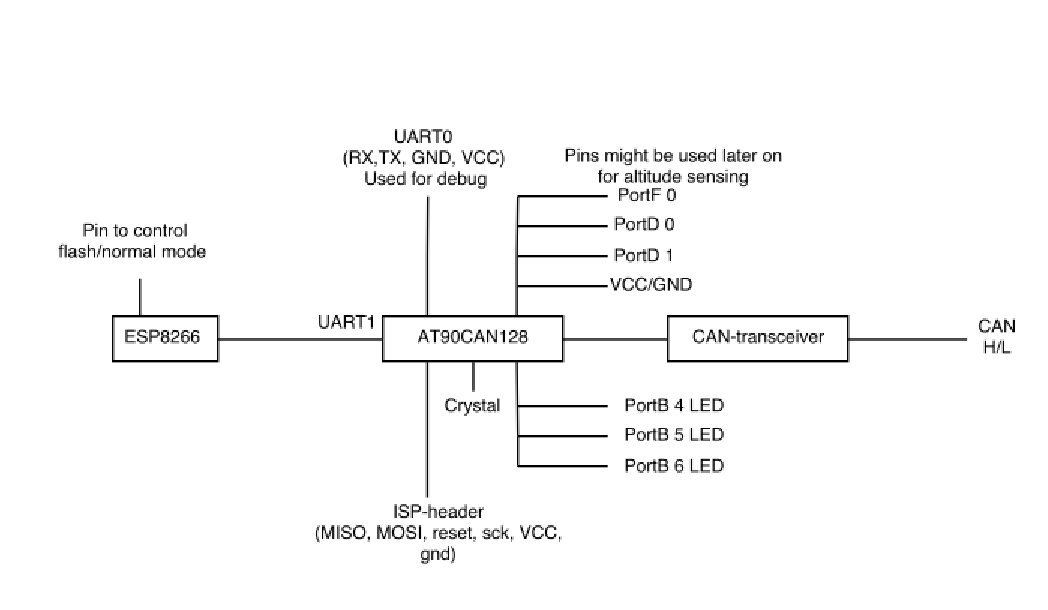
\includegraphics[width=1\textwidth]{graphics/PCB_block_v3.eps}
    \caption{Block schematic of the WIFI-extentionboard developed to AQ M4}
    \label{fig:PCB_block}
\end{figure}

\subsubsection{ATmega}
\subsubsection{Wireless Communication}
An important part of the hardware is the wireless communication used between the PC and the drones.
The wireless communication module has severel requirements it needs to fulfill in order to make the whole system work as expected. A comparison table has been made in table \ref{tab:compare_table_wireless_communication} to find the wireless communication module that is best suited for the task. \\
The following wireless modules where considered and compared.
\begin{itemize}
	\item \textbf{ESP8266}
\end{itemize}

ESP8266 is a generel purpose 32 bit SOC with integrated WIFI 802.11 b/g/n support and buildin TCP/IP stack. It can be setup its own access point or it can connect to an existing wireless network.
It runs at 80MHz and can be flashed with a custom firmware. 
The SOC is sold as modules with different pinouts and features such as extra flash memory \footnote{\url{https://www.olimex.com/Products/IoT/MOD-WIFI-ESP8266/open-source-hardware}} and different antennas.
The chip has been on the marked for about two years and costs approximately 7\$. 
It has been widely used in DIY-projects due to its low price and because it requires a minimum of network knowledge to get up and running.\footnote{\url{http://www.esp8266.com/} - 43.000 posts in forum} When the SOC is shipped, it comes with a preloaded firmware which either accepts AT commands or LUA scripting depending on the version of the module. These simple programming interfaces makes it quick and easy to interface the cheap. \\
This leads to a large community where most of the problems have been found and solved already. Arduino has been ported to ESP8266 which makes it even easier to get it up and running. Their official Arduino GitHub has 2125 commits on their master branch at the time of writing\footnote{\url{https://github.com/esp8266/Arduino}} \\

\begin{itemize}
	\item \textbf{EMW3165}
\end{itemize}
EMW3165 is a SOC much like the ESP8266 supporting 802.11 b/g/n WIFI with buildin TCP/IP stack. As with ESP8266 it supports setting up an access point aswell as connecting to an existing network. It has a Cortex-M4 $\mu$C which run at 100MHz. 
It supports custom firmware and can be aswell be bought as different modules with different pinouts and antennas.
It differentiates itself from the ESP8266 by its higher frequency its 5 volts compatible pins \footnote{\url{https://hackadaycom.files.wordpress.com/2015/07/emw3165.pdf}} which makes it easier to connect other hardware which run 5 volt without the need of a logic level shifter. It has been on the marked for only one year and costs approximately 9\$. Since it is a newer board than ESP8266 it has not been used in the same number of applications and thereby has a smaller community behind\footnote{\url{http://www.emw3165.com/} - 200 posts in forum }. Their most active GitHub has 147 commits on their master branch at the time of writing\footnote{\url{https://github.com/SmartArduino/WiFiMCU}}.

\begin{itemize}
	\item \textbf{nRF51822}
\end{itemize}
nRF51822 is also a SOC, but it is using Bluetooth instead of WIFI. The nRF51822 $\mu$C is implementing BLE which is a power efficient way of sending and receiving data. The chip supports broadcasting which could be used in this project. The $\mu$C can be bought as a standalone component or mounted on modules as the two other $\mu$Cs. Different modules offers different types of antenna connectors or buildin antenna on the PCB. It has not been possible to find an Arduino ported firmware that supports this $\mu$C. To write a firmware for the $\mu$C it has to be done using Nordic Semiconductor's proprietary SDK. 


\begin{itemize}
	\item \textbf{XBee}
\end{itemize}
XBee is a module that implements the Zbee standard. The Xbee modules work as a wireless serial connection. The Xbee modules supports mesh networking which means the modules by themself figure out which module is closest and makes the connection. This idea makes sense in this application since there will be multiple drones and one computer. If one drone gets too far from the PC, it can just connect to one of the other drones closer to the PC.\\
The Xbee solution is ready to use and requires a minimum of programming to get up and running. The modules also support GPIO for digital in and output and analog input.

\Mathias{ '\'footmotemark til at referere til samme fodnote flere gange}
\begin{table}[H]
	\centering
	\begin{tabular}{@{}|l|l|l|l|l|l|l|l|@{}}
		\toprule
		\textbf{Product} & \textbf{Size} & \textbf{Weight} & \textbf{Price} & \textbf{Documentation} &  \textbf{Range}  & \textbf{Score} \\ \midrule
		ESP8266   &  24x16mm\footnote{\url{https://www.mikrocontroller.net/attachment/243558/fcc\_11.pdf}} \hfill\{7\} & 1.5g\footnote{Measured by author on chemistry weight} \hfill\{8\} &   7.5\$\footnote{\url{http://www.seeedstudio.com/depot/ESP8266-based-WiFi-module-SPI-supported-p-2486.html}}    &   \hfill\{9\}        &        &                		\\ \midrule
		EMW3165   &  32x16mm\footnote{\url{https://hackadaycom.files.wordpress.com/2015/07/emw3165.pdf}} \hfill\{6\}  & 5g\footnote{\url{http://www.seeedstudio.com/depot/EMW3165-CortexM4-based-WiFi-SoC-Module-p-2488.html}} \hfill\{2\} &  9\$\footnote{\url{http://www.seeedstudio.com/depot/EMW3165-CortexM4-based-WiFi-SoC-Module-p-2488.html}}   &    \hfill\{3\}	        &        &                		\\ \midrule
		nRF51822  &  18x10mm\footnote{\url{http://www.fanstel.com/Product/bluenor.html}} \hfill\{8\}  & 3g\footnote{\url{http://www.seeedstudio.com/depot/MDBT40P\%C2\%A0\%C2\%A0nRF51822\%C2\%A0based\%C2\%A0BLE\%C2\%A0module-p-2503.html}} \hfill\{0\}  &  7.5\$  & \hfill\{2\} 	        &   30 Meters\footnote{\url{https://dl.dropboxusercontent.com/u/54939426/Fanstel_BT600.pdf}} \hfill\{9\}     &                		\\ \midrule
		XBee      &  24.38x27.61mm \footnote{\url{http://www.digi.com/products/xbee-rf-solutions/modules/xbee-802-15-4\#specifications}} \{3\} & 3g \footnote{\url{http://www.digi.com/products/xbee-rf-solutions/modules/xbee-802-15-4\#specifications}} \hfill\{4\} &   25\$\footnote{\url{https://www.sparkfun.com/products/11215}}    &     \hfill\{9\}      &            91 Meters\footnote{\url{https://www.sparkfun.com/pages/xbee_guide}}  \hfill\{9\}  &                    \\ \bottomrule
	\end{tabular}
	\caption{Comparisontable used to compare different wireless 		communication modules}
	\label{tab:compare_table_wireless_communication}
\end{table}
\Mathias{vægt på ESP til 3 gram med link - det er hvad der er oplyst. Efterfølgende skrive at det er vejet til 1.51 gram(hen mod slutningen)}
The products compared in \ref{tab:compare_table_wireless_communication} are chosen to have approximately same specs. Onboard antenna, breakout for easy pin access.

\subsubsection{Pins}
A few pins where made available through solder pads for easy access if needed later on.

The following pins where available as solder pads:
\begin{itemize}
	\item PortF 0 - Alternative function as ADC, channel 0
	\item PortD 0 - Alternative function as interrupt, INT0
	\item PortD 1 - Alternative function as interrupt, INT1
\end{itemize}
In case the onboard baromter isn't accurate enough, an alternative distance could be used to measure the drones altitude with respect to the ground.
PortF0 has been made available since some distance sensors give output as an analogue value. 
An example of such sensor is an Infrared proximity sensor.\footnote{\url{http://www.sharpsma.com/webfm\_send/1208}} \\
As an alternative type of distance sensor, a ultrasoinc could be used such as HCSR04.
As output it gives a binary output with high-time proportional with the distance.\footnote{\url{http://www.micropik.com/PDF/HCSR04.pdf}}.
To detect the high-time, one of PortD1/0 would be useful. \\

Which type of sensor suits best as a distance sensor to provice altitude information to the drone is ouf of the scope of this report. The PCB has just been made ready to different types of sensors.

\subsubsection{Debug/ISP}
In the final schematic UART0 and ISP pins where combined in one pinheader for easy access through one cable. \Mathias{Refer to image of board}
To program the AtMega the ISP pins where required to be easy accessable. 
UART0 was made accessable to be used as debug and programming of the ESP8266 board.
The plan was to setup the AtMega as UART passthrough from UART0 to UART1.
Due to a mistake\footnote{The wrong pair of MISO/MOSI pins where made available in the ISP-header. The correct pair of MISO/MOSI is also RXD0/TXD0 as alternative function} in the final schematic, both UART0 and UART1 where made accessable trough the ISP/debug header. 
This ended up making it easier to program the ESP8266-board without using the AtMega as UART passthrough.

ESP noteS:
 - GPIO15 = bootmode, low for ...
 - GPIO0 = flash mode
 
 
 https://zoetrope.io/tech-blog/esp8266-bootloader-modes-and-gpio-state-startup
